\section{Seeding by RF Noise} \label{Seed}

Seeding is important in RNG designs as it is fundamental to the randomness of PRNG. CC2538 suggests in its manual to  use the RF core to generate sample seed, as quote as:(Section 16.2.2 in CC2538 User's Guide\cite{CC2538Manual})
\begin{quote}
For the CC2538, when a random value is required, writing the SOC\_ADC\_RNDL register with random bits from the IF\_ADC in the RF receive path seeds the LFSR.
\end{quote}
and: (Section 23.12 in CC2538 User's Guide\cite{CC2538Manual})
\begin{quote}
Single random bits from either the I or Q channel can be read from the RFRND register.
\end{quote}
In case of Contiki, the driver only used the bits generated in I channel.

For the randomness of this seeding method, the manual\cite{CC2538Manual} reported: (Section 23.12 in CC2538 User's Guide\cite{CC2538Manual})
\begin{quote}
Randomness tests show good results for this module. However, a slight DC component exists. In a simple test where the RFRND.IRND register was read a number of times and the data was grouped into bytes, about 20 million bytes were read. When interpreted as unsigned integers between 0 and 255, the mean value was 127.6518, which indicates that there is a DC component.
...
For the first 20 million individual bits, the probability of a 1 is $P(1) = 0.500602$ and $P(0) = 1 - P(1) = 0.499398$.
\end{quote}

Their test results are shown in \Cref{SeedResult}.

\begin{figure}[!t]
\centering
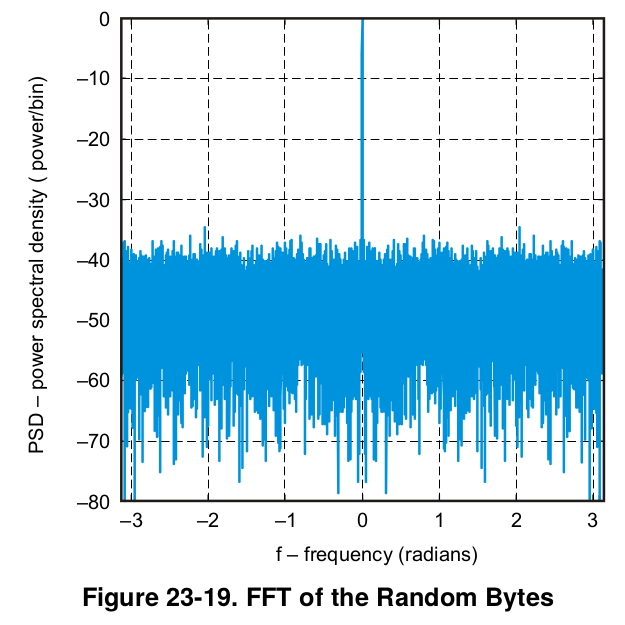
\includegraphics[width=2.5in]{fig/CC2538_Seed1.png}
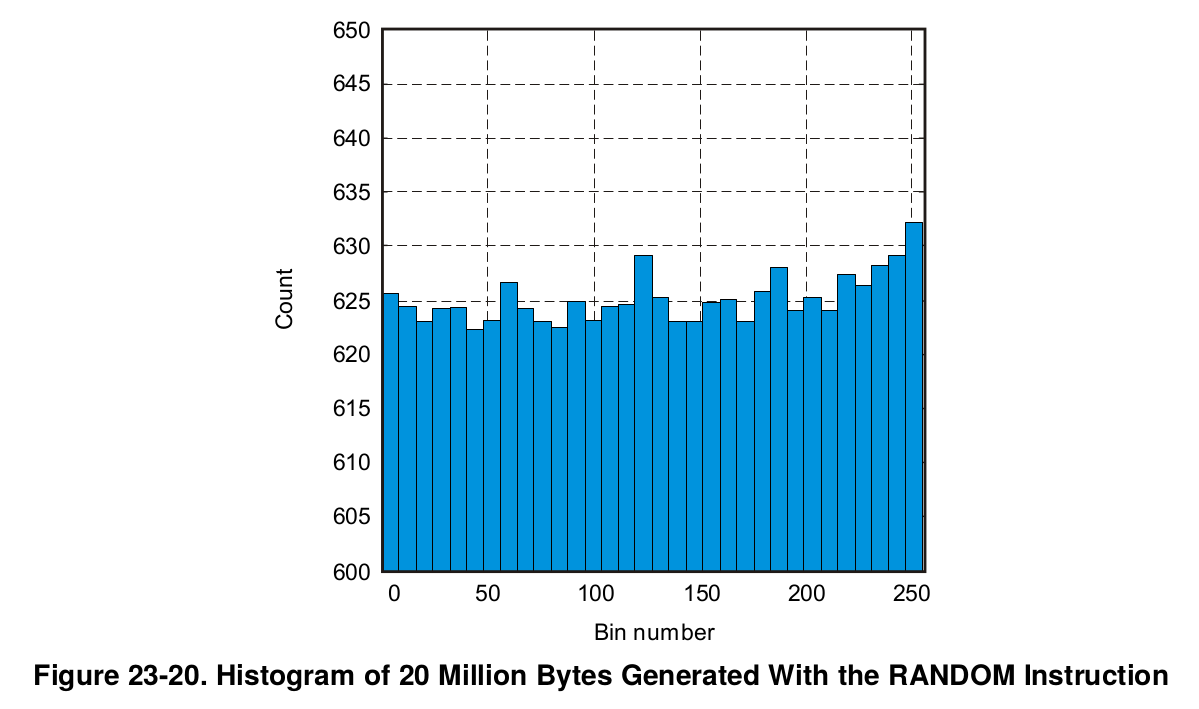
\includegraphics[width=2.5in]{fig/CC2538_Seed2.png}
\caption{RF core seeding result, from CC2538 User's Guide}
\label{SeedResult}
\end{figure}

To further verify the randomness of this seeding method, we applied the NIST Statistical Test Suite\cite{NISTTest} on 13263600 bits sampled by this seeding method using our application in \cite{prngtest}. Since each read to RFRND generates only $1$ bit, we concatenated all bits into one bit stream of length $13263600$. The bits has passed all tests in the NIST test suite, with $P(0) = 0.49995001$ and $P(1) = 0.50004999$. The full report and raw data are applicable at \cite{prngtest}.

Despite the good randomness of the seed, sampling from RF noise remains sceptical from a security perspective as such physical source can be easily tampered remotely by sending signal wave to the device.

The released documents did not explain further details of how the output of IF\_ADC in the I/Q channel of receive path is translated to a random bit. We have neither found any open document describes  the RF design of CC2538. However, we also noticed the same RNG design has been applied on several product in TI's SimpleLink\texttrademark series.